%%%%%%%%%%%%%%%%%%%%%%%%%%%%%%%%%%%%%%%%%%%%%%%%%%%%%%%%%%%%%%%%%%%%%%%%%%%%%%%%
%%%%%%%%%%%%%%%%%%%%%%%%%%%%%%%%%%%%%%%%%%%%%%%%%%%%%%%%%%%%%%%%%%%%%%%%%%%%%%%%
%
% A general frame for lecture slides and lecture notes in one file
% using LaTeX beamer
%
%%%%%%%%%%%%%%%%%%%%%%%%%%%%%%%%%%%%%%%%%%%%%%%%%%%%%%%%%%%%%%%%%%%%%%%%%%%%%%%%
%%%%%%%%%%%%%%%%%%%%%%%%%%%%%%%%%%%%%%%%%%%%%%%%%%%%%%%%%%%%%%%%%%%%%%%%%%%%%%%%
\documentclass[ignorenonframetext,11pt]{beamer}
%\usepackage[ngerman]{babel}
%\usepackage[T1]{fontenc}
\usepackage[utf8]{inputenc}
\usepackage{lmodern}
\usepackage{amsmath,amssymb,amsfonts}


% only presentation
\mode<presentation>
{
  \usetheme{default}
%  \usecolortheme{crane}
  \setbeamercovered{transparent}
%  \setlength{\parindent}{0pt}
%  \setlength{\parskip}{1.35ex plus 0.5ex minus 0.3ex}
%  \usefonttheme{structuresmallcapsserif}
  \usefonttheme{structurebold}
  \setbeamertemplate{theorems}[numbered]
  \usepackage{amscd}
}

% all after
\usepackage{tikz}
\usetikzlibrary{patterns}
\usepackage{pgfplots,adjustbox}
\usepackage{eurosym}
\usepackage{graphicx}
\usepackage{multimedia}
\usepackage{psfrag}
\usepackage{listings}
\lstset{language=C++, basicstyle=\ttfamily,
  keywordstyle=\color{black}\bfseries, tabsize=4, stringstyle=\ttfamily,
  commentstyle=\it, extendedchars=true, escapeinside={/*@}{@*/}}
\usepackage{curves}
%\usepackage{epic}
\usepackage{calc}
%\usepackage{picinpar}
%\usepackage{fancybox}
%\usepackage{xspace}
\usepackage{enumerate}
\usepackage{algpseudocode}
\usepackage{color}
\usepackage{bold-extra}
\usepackage{bm}
\usepackage{stmaryrd}
%\usepackage[squaren]{SIunits}
\usepackage{nicefrac}

\usepackage{fancyvrb,bbm,xspace}
\usepackage{lmodern}
\usepackage{fancyvrb,bbm,xspace}
\usepackage[binary-units]{siunitx}
\usepackage{xcolor,tabu}

\definecolor{niceblue}{rgb}{0.122,0.396,0.651}   %% 31, 101, 166 or #1F65A6
\definecolor{niceorange}{RGB}{255,205,86}        %% #FFCD56
\definecolor{nicered}{RGB}{220,20,60}                      %% rgb(220, 20, 60)
\definecolor{niceteal}{HTML}{00A9AB}
\definecolor{niceviolet}{HTML}{820080}

\definecolor{niceblueLight}{HTML}{91CAFB}
\definecolor{niceblueVeryLight}{HTML}{DDEFFF}

\usepackage{dsfont}

%\newcommand{\hlineabove}{\rule{0pt}{2.6ex}}
%\newcommand{\hlinebelow}{\rule[-1.2ex]{0pt}{0pt}}

%\usecolortheme[RGB={37,75,123}]{structure}
% \definecolor{structurecolor}{rgb}{0.905,0.318,0.071}

% \setbeamercolor{frametitle}{fg=black,bg=}
% \setbeamercolor{sidebar left}{fg=,bg=}

% \setbeamertemplate{headline}{\vskip4em}
% \setbeamersize{sidebar width left=.9cm}

% \setbeamertemplate{navigation symbols}{}
%\setbeamertemplate{blocks}[rounded][shadow=true]
%\setbeamertemplate{itemize items}[square]

\mode<presentation>
{
\theoremstyle{definition}
}
\newtheorem{Def}{Definition}%[section]
\newtheorem{Exm}[Def]{Example}
\newtheorem{Lem}[Def]{Lemma}
\newtheorem{Rem}[Def]{Remark}
\newtheorem{Rul}[Def]{Rule}
\newtheorem{Thm}[Def]{Theorem}
\newtheorem{Cor}[Def]{Corollary}
\newtheorem{Obs}[Def]{Observation}
\newtheorem{Ass}[Def]{Assumption}
\newtheorem{Pro}[Def]{Property}
\newtheorem{Alg}[Def]{Algorithm}
\newtheorem{Prp}[Def]{Proposition}
\newtheorem{Lst}[Def]{Listing}

% Delete this, if you do not want the table of contents to pop up at
% the beginning of each subsection:
\AtBeginSection[]
{
  \begin{frame}<beamer>
    \frametitle{Contents}
    \tableofcontents[sectionstyle=show/shaded,subsectionstyle=hide/hide/hide]
%\tableofcontents[currentsection]
  \end{frame}
}

% Title definition
\mode<presentation>
{
  \title{DUNE PDELab Tutorial 04\\
  {\small Finite Elements for the Wave Equation}}
  \author{Peter Bastian \and Steffen Müthing}
  \institute[]
  {
   Interdisziplinäres Zentrum für Wissenschaftliches Rechnen\\
   Im Neuenheimer Feld 205, D-69120 Heidelberg \\[6pt]
  }
  \date[\today]{\today}
}


% logo nach oben
\mode<presentation>
{
% No navigation symbols and no lower logo
\setbeamertemplate{sidebar right}{}

% logo
\newsavebox{\logobox}
\sbox{\logobox}{%
    \hskip\paperwidth%
    \rlap{%
      % putting the logo should not change the vertical possition
      \vbox to 0pt{%
        \vskip-\paperheight%
        \vskip0.35cm%
        \llap{\insertlogo\hskip0.1cm}%
        % avoid overfull \vbox messages
        \vss%
      }%
    }%
}

\addtobeamertemplate{footline}{}{%
    \usebox{\logobox}%
}
}

%%%%%%%%%%%%%%%%%%%%%%%%%%%%%%%%%%%%%%%%%%%%%%%%%%%%%%%%%%%%%%%%%%%%%%%%%%%%%%%%
%%%%%%%%%%%%%%%%%%%%%%%%%%%%%%%%%%%%%%%%%%%%%%%%%%%%%%%%%%%%%%%%%%%%%%%%%%%%%%%%
%
% now comes the individual stuff lecture by lecture
%
%%%%%%%%%%%%%%%%%%%%%%%%%%%%%%%%%%%%%%%%%%%%%%%%%%%%%%%%%%%%%%%%%%%%%%%%%%%%%%%%
%%%%%%%%%%%%%%%%%%%%%%%%%%%%%%%%%%%%%%%%%%%%%%%%%%%%%%%%%%%%%%%%%%%%%%%%%%%%%%%%

\begin{document}

\frame{\titlepage}

%%%%%%%%%%%%%%%%%%%%%%%%%%%%%%%%%%%%%%%%%%%%%%%%%%%%%%%%%%%%%%%%%%%%%%%%%%%%%%%%
%%%%%%%%%%%%%%%%%%%%%%%%%%%%%%%%%%%%%%%%%%%%%%%%%%%%%%%%%%%%%%%%%%%%%%%%%%%%%%%%


\begin{frame}
\frametitle{Example Problem}
 In this tutorial we solve the wave equation formulated as a first order
in time system. This way the example serves as a model for the
treatment of systems of partial differential equations in PDELab.

\begin{subequations}
\label{eq:WaveEquation}
\begin{align}
\partial_{tt} u-c^2\Delta u  &= 0 &&\text{in $\Omega\times\Sigma$},\\
u &= 0 &&\text{on $\partial\Omega$},\\
u &= q &&\text{at $t=0$},\\
\partial_t u &= w &&\text{at $t=0$},
\end{align}
\end{subequations}
where $c$ is the speed of sound.
\end{frame}
\begin{frame}
Renaming $u_0=u$ and introducing $u_1=\partial_t u_0 =\partial_t u$ we can write the wave equation as a system of two equations:
\begin{subequations}
\label{eq:SystemForm1}
\begin{align}
\partial_t u_1 - c^2\Delta u_0 &=0 &&\text{in $\Omega\times\Sigma$}, \label{eq:2a}\\
\partial_t u_0 - u_1 &=0 &&\text{in $\Omega\times\Sigma$}, \label{eq:2b}\\
u_0 &= 0 &&\text{on $\partial\Omega$},\\
u_1 &= 0 &&\text{on $\partial\Omega$},\\
u_0 &= q &&\text{at $t=0$},\\
u_1 &= w &&\text{at $t=0$}.
\end{align}
\end{subequations}
Since $u_0=u=0$ on the boundary we also have $\partial_t u = u_1 = 0$ on the boundary.
Alternatively, omit the boundary condition on $u_1$.
\end{frame}


\begin{frame}
\frametitle{Alternative Formulations (I)}
Eriksson et al. in \cite{Eriksson} apply the Laplacian to
equation \eqref{eq:2b}
\begin{equation}
\Delta \partial_t u_0 - \Delta u_1 = 0
\end{equation} \label{eq:Eriksson}
which has advantages for energy conservation but requires additional smoothness
properties.
\end{frame}

\begin{frame}
\frametitle{Alternative Formulations (II)}
Introduce the abbreviations
$q=\partial_t u$ and $w=-\nabla u$, so $\partial_{tt} u - c^2 \Delta u =
\partial_{tt} u - c^2 \nabla\cdot\nabla u = \partial_{t} q + c^2 \nabla\cdot w = 0$.
Taking partial derivatives of the introduced variables we obtain $\partial_{x_i} q=
\partial_{x_i} \partial_t u = \partial_t \partial_{x_i}  u = - \partial_t w_i$. This results
in a first-order hyperbolic system of PDEs for $q$ and $w$
\begin{align*}
\partial_t q + c^2 \nabla\cdot w &= 0\\
\partial_t w + \nabla q &= 0
\end{align*}
which are called equations of linear acoustics \cite{LeVeque}. This formulation
is physically more relevant. It can be modified to handle discontinuous material
properties and supports upwind finite volume methods.
\end{frame}


\begin{frame}
\frametitle{Weak Formulation}

Multiplying \eqref{eq:2a}
with the test function $v_0$ and \eqref{eq:2b} with the test function $v_1$
and using integration by parts we arrive at the weak formulation: Find $(u_0(t),u_1(t))\in
U_0\times U_1$ s.t.
\begin{align}
  d_t (u_1,v_0)_{0,\Omega} + c^2 (\nabla u_0, \nabla v_0)_{0,\Omega} &=
  0 \quad \forall v_0 \in U_0 \notag \\
  d_t (u_0,v_1)_{0,\Omega} - (u_1,v_1)_{0,\Omega} &= 0 \quad \forall
  v_1 \in U_1 \label{eq:WeakFormSystem}
\end{align}
where we used the notation of the $L^2$ inner product $(u,v)_{0,\Omega} = \int_\Omega
u v \, dx$.
\end{frame}

\begin{frame}
An equivalent formulation to (\ref{eq:WeakFormSystem}) that
hides the system structure reads as follows:
\begin{equation}
\label{eq:WeakForm}
\begin{split}
d_t &\left[ (u_0,v_1)_{0,\Omega} + (u_1,v_0)_{0,\Omega}\right] \\
&\hspace{6mm}+ \left[ c^2 (\nabla u_0,\nabla v_0)_{0,\Omega} -(u_1,v_1)_{0,\Omega} \right] = 0
\quad \forall (v_0,v_1)\in U_0\times U_1
\end{split}
\end{equation}
With the latter we readily identify the temporal and spatial residual
forms:
\begin{align}
m^{\text{WAVE}}((u_0,u_1),(v_0,v_1)) &= (u_0,v_1)_{0,\Omega} + (u_1,v_0)_{0,\Omega},
\label{eq:TemporalResForm}\\
r^{\text{WAVE}}((u_0,u_1),(v_0,v_1)) &= c^2 (\nabla u_0,\nabla
v_0)_{0,\Omega} - (u_1,v_1)_{0,\Omega} \; . \label{eq:SpatialResForm}
\end{align}
\end{frame}


\begin{frame}{Trees of Function spaces}
  \begin{columns}
    \begin{column}{0.6\textwidth}
$U = \bigl(V(\Omega_S)\bigr)^d \times P(\Omega_S) \times \Phi(\Omega_D)$

\begin{itemize}
\item Computer science way of representing mathematical  expressions: \structure{Trees}
\item Expose internal nodes to users
  \begin{itemize}
  \item {\small Enable recursive bottom-up construction}
  \item {\small Extract subtrees to pass to legacy subproblem code}
  \end{itemize}
\item Tree structure mostly static after construction
  \begin{itemize}
  \item {\small Nodes are C++ templates with children as template arguments}
  \item {\small Allows extensive compiler optimizations, including inlining of tree traversals}
  \end{itemize}
\end{itemize}

    \end{column}
    \begin{column}{0.4\textwidth}
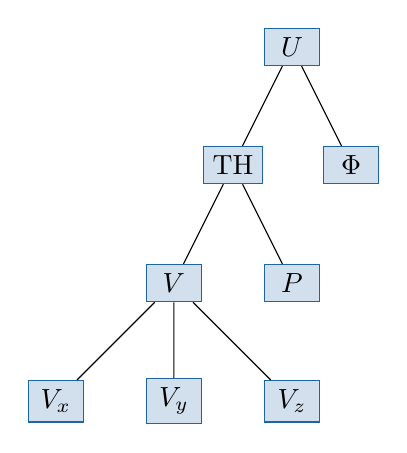
\begin{tikzpicture}
    [every node/.style={draw=niceblue,fill=niceblue!20, minimum width=.7cm}]
  \node {$U$}
  child {
    node {TH}
      child {
        node  {$V$}
        child {
          node  {$V_x$}
        }
        child {
          node  {$V_y$}
        }
        child {
          node  {$V_z$}
        }
      }
      child {
        node  {$P$}
      }
    }
  child {
    node {$\Phi$}
  };
\end{tikzpicture}

    \end{column}
  \end{columns}


\end{frame}

\begin{frame}{Linear Algebra}

    Given an assembled residual $r = \mathcal{R}(\vec{u_0})$ and its Jacobian $A = \nabla\mathcal{R}_h$, we have to solve the linear problem
    \begin{equation*}
      A z = r
    \end{equation*}
    to obtain a correction and calculate $u = u_0 - z$.\\
  \emph{Several options}
  \begin{description}
  \item[Monolithic solve] of $A z = r$
  \end{description}
  \begin{itemize}
  \item No stability problems
  \item Often very difficult with standard iterative solvers
  \end{itemize}
  \begin{description}
  \item[Subdomain Iteration] Exploit problem structure
  \end{description}
\begin{equation*}
  \begin{pmatrix}
    A_L & 0 \\
    0  & A_R \\
  \end{pmatrix}
  \begin{pmatrix}
    z_L \\ z_R \\
  \end{pmatrix}
  =
  \begin{pmatrix}
    r_L \\ r_R \\
  \end{pmatrix}
\end{equation*}
\begin{itemize}
\item Stability can be problematic
\item Does not require monolithic code base
\item Matrix / vector data structures must contain structure for good performance
\end{itemize}
\end{frame}



\begin{frame}{Index Merging -- Example}
  \begin{columns}
    \begin{column}{0.5\textwidth}
      \begin{itemize}
      \item Two $Q_1$ spaces on common mesh
      \item Each space has canonical order defined by vertex iteration
      \item Two merging strategies
        \structure{Lexicographic:} Preserve structure of individual problems, separate matrix blocks for coupling\\
        \structure{Interleaved:} Regard problem as vector-valued version of scalar problem
      \end{itemize}
% \tikzexternalenable
% \resizebox{\textwidth}{!}{
% 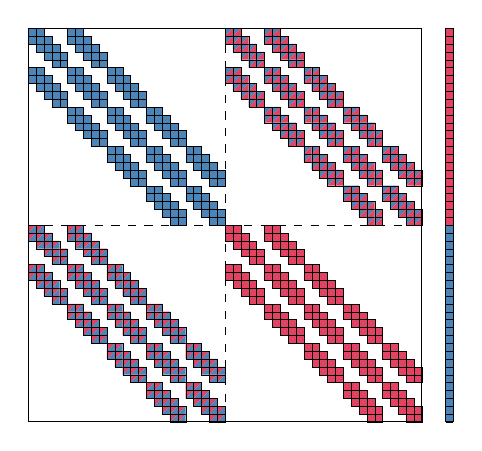
\begin{tikzpicture}

\colorlet{ca}{niceblue!80}
\colorlet{cb}{nicered!80}
\colorlet{cc}{niceorange!90}
\colorlet{cd}{niceviolet!60}

%%% Local Variables:
%%% mode: latex
%%% TeX-master: "../../diss-main"
%%% End:


\foreach \x / \y in {0/0, 0/1, 0/5, 0/6, 1/0, 1/1, 1/2, 1/5, 1/6, 1/7, 2/1, 2/2, 2/3, 2/6, 2/7, 2/8, 3/2, 3/3, 3/4, 3/7, 3/8, 3/9, 4/3, 4/4, 4/8, 4/9, 5/0, 5/1, 5/5, 5/6, 5/10, 5/11, 6/0, 6/1, 6/2, 6/5, 6/6, 6/7, 6/10, 6/11, 6/12, 7/1, 7/2, 7/3, 7/6, 7/7, 7/8, 7/11, 7/12, 7/13, 8/2, 8/3, 8/4, 8/7, 8/8, 8/9, 8/12, 8/13, 8/14, 9/3, 9/4, 9/8, 9/9, 9/13, 9/14, 10/5, 10/6, 10/10, 10/11, 10/15, 10/16, 11/5, 11/6, 11/7, 11/10, 11/11, 11/12, 11/15, 11/16, 11/17, 12/6, 12/7, 12/8, 12/11, 12/12, 12/13, 12/16, 12/17, 12/18, 13/7, 13/8, 13/9, 13/12, 13/13, 13/14, 13/17, 13/18, 13/19, 14/8, 14/9, 14/13, 14/14, 14/18, 14/19, 15/10, 15/11, 15/15, 15/16, 15/20, 15/21, 16/10, 16/11, 16/12, 16/15, 16/16, 16/17, 16/20, 16/21, 16/22, 17/11, 17/12, 17/13, 17/16, 17/17, 17/18, 17/21, 17/22, 17/23, 18/12, 18/13, 18/14, 18/17, 18/18, 18/19, 18/22, 18/23, 18/24, 19/13, 19/14, 19/18, 19/19, 19/23, 19/24, 20/15, 20/16, 20/20, 20/21, 21/15, 21/16, 21/17, 21/20, 21/21, 21/22, 22/16, 22/17, 22/18, 22/21, 22/22, 22/23, 23/17, 23/18, 23/19, 23/22, 23/23, 23/24, 24/18, 24/19, 24/23, 24/24}
{
  \filldraw[fill=ca,ultra thin] (0.1*\x,-0.1*\y) rectangle ++(0.1,-0.1);
}

\foreach \x / \y in {25/25, 25/26, 25/30, 25/31, 26/25, 26/26, 26/27, 26/30, 26/31, 26/32, 27/26, 27/27, 27/28, 27/31, 27/32, 27/33, 28/27, 28/28, 28/29, 28/32, 28/33, 28/34, 29/28, 29/29, 29/33, 29/34, 30/25, 30/26, 30/30, 30/31, 30/35, 30/36, 31/25, 31/26, 31/27, 31/30, 31/31, 31/32, 31/35, 31/36, 31/37, 32/26, 32/27, 32/28, 32/31, 32/32, 32/33, 32/36, 32/37, 32/38, 33/27, 33/28, 33/29, 33/32, 33/33, 33/34, 33/37, 33/38, 33/39, 34/28, 34/29, 34/33, 34/34, 34/38, 34/39, 35/30, 35/31, 35/35, 35/36, 35/40, 35/41, 36/30, 36/31, 36/32, 36/35, 36/36, 36/37, 36/40, 36/41, 36/42, 37/31, 37/32, 37/33, 37/36, 37/37, 37/38, 37/41, 37/42, 37/43, 38/32, 38/33, 38/34, 38/37, 38/38, 38/39, 38/42, 38/43, 38/44, 39/33, 39/34, 39/38, 39/39, 39/43, 39/44, 40/35, 40/36, 40/40, 40/41, 40/45, 40/46, 41/35, 41/36, 41/37, 41/40, 41/41, 41/42, 41/45, 41/46, 41/47, 42/36, 42/37, 42/38, 42/41, 42/42, 42/43, 42/46, 42/47, 42/48, 43/37, 43/38, 43/39, 43/42, 43/43, 43/44, 43/47, 43/48, 43/49, 44/38, 44/39, 44/43, 44/44, 44/48, 44/49, 45/40, 45/41, 45/45, 45/46, 46/40, 46/41, 46/42, 46/45, 46/46, 46/47, 47/41, 47/42, 47/43, 47/46, 47/47, 47/48, 48/42, 48/43, 48/44, 48/47, 48/48, 48/49, 49/43, 49/44, 49/48, 49/49}
{
  \filldraw[fill=cb,ultra thin] (0.1*\x,-0.1*\y) rectangle ++(0.1,-0.1);
}

\foreach \x / \y in {0/25, 0/26, 0/30, 0/31, 1/25, 1/26, 1/27, 1/30, 1/31, 1/32, 2/26, 2/27, 2/28, 2/31, 2/32, 2/33, 3/27, 3/28, 3/29, 3/32, 3/33, 3/34, 4/28, 4/29, 4/33, 4/34, 5/25, 5/26, 5/30, 5/31, 5/35, 5/36, 6/25, 6/26, 6/27, 6/30, 6/31, 6/32, 6/35, 6/36, 6/37, 7/26, 7/27, 7/28, 7/31, 7/32, 7/33, 7/36, 7/37, 7/38, 8/27, 8/28, 8/29, 8/32, 8/33, 8/34, 8/37, 8/38, 8/39, 9/28, 9/29, 9/33, 9/34, 9/38, 9/39, 10/30, 10/31, 10/35, 10/36, 10/40, 10/41, 11/30, 11/31, 11/32, 11/35, 11/36, 11/37, 11/40, 11/41, 11/42, 12/31, 12/32, 12/33, 12/36, 12/37, 12/38, 12/41, 12/42, 12/43, 13/32, 13/33, 13/34, 13/37, 13/38, 13/39, 13/42, 13/43, 13/44, 14/33, 14/34, 14/38, 14/39, 14/43, 14/44, 15/35, 15/36, 15/40, 15/41, 15/45, 15/46, 16/35, 16/36, 16/37, 16/40, 16/41, 16/42, 16/45, 16/46, 16/47, 17/36, 17/37, 17/38, 17/41, 17/42, 17/43, 17/46, 17/47, 17/48, 18/37, 18/38, 18/39, 18/42, 18/43, 18/44, 18/47, 18/48, 18/49, 19/38, 19/39, 19/43, 19/44, 19/48, 19/49, 20/40, 20/41, 20/45, 20/46, 21/40, 21/41, 21/42, 21/45, 21/46, 21/47, 22/41, 22/42, 22/43, 22/46, 22/47, 22/48, 23/42, 23/43, 23/44, 23/47, 23/48, 23/49, 24/43, 24/44, 24/48, 24/49}
{
  \fill[cb] (0.1*\x,-0.1*\y) -- ++(0.1,0) -- ++(-0.1,-0.1) --cycle;
  \fill[ca] (0.1*\x+0.1,-0.1*\y) -- ++(0,-0.1) -- ++(-0.1,0) --cycle;
  \draw[ultra thin] (0.1*\x,-0.1*\y) rectangle ++(0.1,-0.1);
}

\foreach \x / \y in {25/0, 25/1, 25/5, 25/6, 26/0, 26/1, 26/2, 26/5, 26/6, 26/7, 27/1, 27/2, 27/3, 27/6, 27/7, 27/8, 28/2, 28/3, 28/4, 28/7, 28/8, 28/9, 29/3, 29/4, 29/8, 29/9, 30/0, 30/1, 30/5, 30/6, 30/10, 30/11, 31/0, 31/1, 31/2, 31/5, 31/6, 31/7, 31/10, 31/11, 31/12, 32/1, 32/2, 32/3, 32/6, 32/7, 32/8, 32/11, 32/12, 32/13, 33/2, 33/3, 33/4, 33/7, 33/8, 33/9, 33/12, 33/13, 33/14, 34/3, 34/4, 34/8, 34/9, 34/13, 34/14, 35/5, 35/6, 35/10, 35/11, 35/15, 35/16, 36/5, 36/6, 36/7, 36/10, 36/11, 36/12, 36/15, 36/16, 36/17, 37/6, 37/7, 37/8, 37/11, 37/12, 37/13, 37/16, 37/17, 37/18, 38/7, 38/8, 38/9, 38/12, 38/13, 38/14, 38/17, 38/18, 38/19, 39/8, 39/9, 39/13, 39/14, 39/18, 39/19, 40/10, 40/11, 40/15, 40/16, 40/20, 40/21, 41/10, 41/11, 41/12, 41/15, 41/16, 41/17, 41/20, 41/21, 41/22, 42/11, 42/12, 42/13, 42/16, 42/17, 42/18, 42/21, 42/22, 42/23, 43/12, 43/13, 43/14, 43/17, 43/18, 43/19, 43/22, 43/23, 43/24, 44/13, 44/14, 44/18, 44/19, 44/23, 44/24, 45/15, 45/16, 45/20, 45/21, 46/15, 46/16, 46/17, 46/20, 46/21, 46/22, 47/16, 47/17, 47/18, 47/21, 47/22, 47/23, 48/17, 48/18, 48/19, 48/22, 48/23, 48/24, 49/18, 49/19, 49/23, 49/24}
{
  \fill[ca] (0.1*\x,-0.1*\y) -- ++(0.1,0) -- ++(-0.1,-0.1) --cycle;
  \fill[cb] (0.1*\x+0.1,-0.1*\y) -- ++(0,-0.1) -- ++(-0.1,0) --cycle;
  \draw[ultra thin] (0.1*\x,-0.1*\y) rectangle ++(0.1,-0.1);
}

\fill[cb] (5.3,0) rectangle ++(0.1,-2.5);
\fill[ca] (5.3,-2.5) rectangle ++(0.1,-2.5);
\draw (5.3,0) rectangle ++(0.1,-5);

\foreach \x in {0,1,...,50}
{
  %\draw (0.1*\x,0) -- ++(0,-5);
  %\draw (0,-0.1*\x) -- ++(5,0);
  \draw[ultra thin] (5.3,-0.1*\x) -- ++(0.1,0);
}

\draw (0,0) rectangle (5,-5);

\draw[dashed,very thin]
  (0,-2.5) -- (5,-2.5)
  (2.5,0) -- (2.5,-5);

\end{tikzpicture}


%%% Local Variables:
%%% mode: latex
%%% TeX-master: "../../diss-main"
%%% End:

% 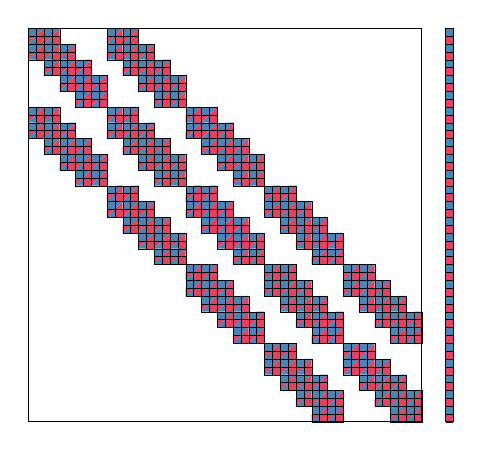
\begin{tikzpicture}

\colorlet{ca}{niceblue!80}
\colorlet{cb}{nicered!80}
\colorlet{cc}{niceorange!90}
\colorlet{cd}{niceviolet!60}

%%% Local Variables:
%%% mode: latex
%%% TeX-master: "../../diss-main"
%%% End:


\foreach \x / \y in {0/0, 0/2, 0/10, 0/12, 2/0, 2/2, 2/4, 2/10,
  2/12, 2/14, 4/2, 4/4, 4/6, 4/12, 4/14, 4/16, 6/4, 6/6, 6/8,
  6/14, 6/16, 6/18, 8/6, 8/8, 8/16, 8/18, 10/0, 10/2, 10/10,
  10/12, 10/20, 10/22, 12/0, 12/2, 12/4, 12/10, 12/12, 12/14,
  12/20, 12/22, 12/24, 14/2, 14/4, 14/6, 14/12, 14/14, 14/16,
  14/22, 14/24, 14/26, 16/4, 16/6, 16/8, 16/14, 16/16, 16/18,
  16/24, 16/26, 16/28, 18/6, 18/8, 18/16, 18/18, 18/26, 18/28,
  20/10, 20/12, 20/20, 20/22, 20/30, 20/32, 22/10, 22/12, 22/14,
  22/20, 22/22, 22/24, 22/30, 22/32, 22/34, 24/12, 24/14, 24/16,
  24/22, 24/24, 24/26, 24/32, 24/34, 24/36, 26/14, 26/16, 26/18,
  26/24, 26/26, 26/28, 26/34, 26/36, 26/38, 28/16, 28/18, 28/26,
  28/28, 28/36, 28/38, 30/20, 30/22, 30/30, 30/32, 30/40, 30/42,
  32/20, 32/22, 32/24, 32/30, 32/32, 32/34, 32/40, 32/42, 32/44,
  34/22, 34/24, 34/26, 34/32, 34/34, 34/36, 34/42, 34/44, 34/46,
  36/24, 36/26, 36/28, 36/34, 36/36, 36/38, 36/44, 36/46, 36/48,
  38/26, 38/28, 38/36, 38/38, 38/46, 38/48, 40/30, 40/32, 40/40,
  40/42, 42/30, 42/32, 42/34, 42/40, 42/42, 42/44, 44/32, 44/34,
  44/36, 44/42, 44/44, 44/46, 46/34, 46/36, 46/38, 46/44, 46/46,
  46/48, 48/36, 48/38, 48/46, 48/48}
{
  \filldraw[fill=ca,ultra thin] (0.1*\x,-0.1*\y) rectangle ++(0.1,-0.1);
}

\foreach \x / \y in {1/1, 1/3, 1/11, 1/13, 3/1, 3/3, 3/5, 3/11,
  3/13, 3/15, 5/3, 5/5, 5/7, 5/13, 5/15, 5/17, 7/5, 7/7, 7/9,
  7/15, 7/17, 7/19, 9/7, 9/9, 9/17, 9/19, 11/1, 11/3, 11/11,
  11/13, 11/21, 11/23, 13/1, 13/3, 13/5, 13/11, 13/13, 13/15,
  13/21, 13/23, 13/25, 15/3, 15/5, 15/7, 15/13, 15/15, 15/17,
  15/23, 15/25, 15/27, 17/5, 17/7, 17/9, 17/15, 17/17, 17/19,
  17/25, 17/27, 17/29, 19/7, 19/9, 19/17, 19/19, 19/27, 19/29,
  21/11, 21/13, 21/21, 21/23, 21/31, 21/33, 23/11, 23/13, 23/15,
  23/21, 23/23, 23/25, 23/31, 23/33, 23/35, 25/13, 25/15, 25/17,
  25/23, 25/25, 25/27, 25/33, 25/35, 25/37, 27/15, 27/17, 27/19,
  27/25, 27/27, 27/29, 27/35, 27/37, 27/39, 29/17, 29/19, 29/27,
  29/29, 29/37, 29/39, 31/21, 31/23, 31/31, 31/33, 31/41, 31/43,
  33/21, 33/23, 33/25, 33/31, 33/33, 33/35, 33/41, 33/43, 33/45,
  35/23, 35/25, 35/27, 35/33, 35/35, 35/37, 35/43, 35/45, 35/47,
  37/25, 37/27, 37/29, 37/35, 37/37, 37/39, 37/45, 37/47, 37/49,
  39/27, 39/29, 39/37, 39/39, 39/47, 39/49, 41/31, 41/33, 41/41,
  41/43, 43/31, 43/33, 43/35, 43/41, 43/43, 43/45, 45/33, 45/35,
  45/37, 45/43, 45/45, 45/47, 47/35, 47/37, 47/39, 47/45, 47/47,
  47/49, 49/37, 49/39, 49/47, 49/49}
{
  \filldraw[fill=cb,ultra thin] (0.1*\x,-0.1*\y) rectangle ++(0.1,-0.1);
}

\foreach \x / \y in {0/1, 0/3, 0/11, 0/13, 2/1, 2/3, 2/5, 2/11,
  2/13, 2/15, 4/3, 4/5, 4/7, 4/13, 4/15, 4/17, 6/5, 6/7, 6/9,
  6/15, 6/17, 6/19, 8/7, 8/9, 8/17, 8/19, 10/1, 10/3, 10/11,
  10/13, 10/21, 10/23, 12/1, 12/3, 12/5, 12/11, 12/13, 12/15,
  12/21, 12/23, 12/25, 14/3, 14/5, 14/7, 14/13, 14/15, 14/17,
  14/23, 14/25, 14/27, 16/5, 16/7, 16/9, 16/15, 16/17, 16/19,
  16/25, 16/27, 16/29, 18/7, 18/9, 18/17, 18/19, 18/27, 18/29,
  20/11, 20/13, 20/21, 20/23, 20/31, 20/33, 22/11, 22/13, 22/15,
  22/21, 22/23, 22/25, 22/31, 22/33, 22/35, 24/13, 24/15, 24/17,
  24/23, 24/25, 24/27, 24/33, 24/35, 24/37, 26/15, 26/17, 26/19,
  26/25, 26/27, 26/29, 26/35, 26/37, 26/39, 28/17, 28/19, 28/27,
  28/29, 28/37, 28/39, 30/21, 30/23, 30/31, 30/33, 30/41, 30/43,
  32/21, 32/23, 32/25, 32/31, 32/33, 32/35, 32/41, 32/43, 32/45,
  34/23, 34/25, 34/27, 34/33, 34/35, 34/37, 34/43, 34/45, 34/47,
  36/25, 36/27, 36/29, 36/35, 36/37, 36/39, 36/45, 36/47, 36/49,
  38/27, 38/29, 38/37, 38/39, 38/47, 38/49, 40/31, 40/33, 40/41,
  40/43, 42/31, 42/33, 42/35, 42/41, 42/43, 42/45, 44/33, 44/35,
  44/37, 44/43, 44/45, 44/47, 46/35, 46/37, 46/39, 46/45, 46/47,
  46/49, 48/37, 48/39, 48/47, 48/49}
{
  \fill[cb] (0.1*\x,-0.1*\y) -- ++(0.1,0) -- ++(-0.1,-0.1) --cycle;
  \fill[ca] (0.1*\x+0.1,-0.1*\y) -- ++(0,-0.1) -- ++(-0.1,0) --cycle;
  \draw[ultra thin] (0.1*\x,-0.1*\y) rectangle ++(0.1,-0.1);
}

\foreach \x / \y in {1/0, 1/2, 1/10, 1/12, 3/0, 3/2, 3/4, 3/10,
  3/12, 3/14, 5/2, 5/4, 5/6, 5/12, 5/14, 5/16, 7/4, 7/6, 7/8,
  7/14, 7/16, 7/18, 9/6, 9/8, 9/16, 9/18, 11/0, 11/2, 11/10,
  11/12, 11/20, 11/22, 13/0, 13/2, 13/4, 13/10, 13/12, 13/14,
  13/20, 13/22, 13/24, 15/2, 15/4, 15/6, 15/12, 15/14, 15/16,
  15/22, 15/24, 15/26, 17/4, 17/6, 17/8, 17/14, 17/16, 17/18,
  17/24, 17/26, 17/28, 19/6, 19/8, 19/16, 19/18, 19/26, 19/28,
  21/10, 21/12, 21/20, 21/22, 21/30, 21/32, 23/10, 23/12, 23/14,
  23/20, 23/22, 23/24, 23/30, 23/32, 23/34, 25/12, 25/14, 25/16,
  25/22, 25/24, 25/26, 25/32, 25/34, 25/36, 27/14, 27/16, 27/18,
  27/24, 27/26, 27/28, 27/34, 27/36, 27/38, 29/16, 29/18, 29/26,
  29/28, 29/36, 29/38, 31/20, 31/22, 31/30, 31/32, 31/40, 31/42,
  33/20, 33/22, 33/24, 33/30, 33/32, 33/34, 33/40, 33/42, 33/44,
  35/22, 35/24, 35/26, 35/32, 35/34, 35/36, 35/42, 35/44, 35/46,
  37/24, 37/26, 37/28, 37/34, 37/36, 37/38, 37/44, 37/46, 37/48,
  39/26, 39/28, 39/36, 39/38, 39/46, 39/48, 41/30, 41/32, 41/40,
  41/42, 43/30, 43/32, 43/34, 43/40, 43/42, 43/44, 45/32, 45/34,
  45/36, 45/42, 45/44, 45/46, 47/34, 47/36, 47/38, 47/44, 47/46,
  47/48, 49/36, 49/38, 49/46, 49/48}
{
  \fill[ca] (0.1*\x,-0.1*\y) -- ++(0.1,0) -- ++(-0.1,-0.1) --cycle;
  \fill[cb] (0.1*\x+0.1,-0.1*\y) -- ++(0,-0.1) -- ++(-0.1,0) --cycle;
  \draw[ultra thin] (0.1*\x,-0.1*\y) rectangle ++(0.1,-0.1);
}

\foreach \x in {0,1,...,24}
{
  \fill[ca] (5.3,-0.2*\x) rectangle ++(0.1,-0.1);
  \fill[cb] (5.3,-0.2*\x-0.1) rectangle ++(0.1,-0.1);
}

\draw (5.3,0) rectangle ++(0.1,-5);

\foreach \x in {0,1,...,50}
{
  %\draw (0.1*\x,0) -- ++(0,-5);
  %\draw (0,-0.1*\x) -- ++(5,0);
  \draw[ultra thin] (5.3,-0.1*\x) -- ++(0.1,0);
}

\draw (0,0) rectangle (5,-5);

\end{tikzpicture}


%%% Local Variables:
%%% mode: latex
%%% TeX-master: "../../diss-main"
%%% End:

% }
% \tikzexternaldisable

    \end{column}
    \begin{column}{0.5\textwidth}
{\Large
\begin{equation*}
U = U_1 \times U_2
\end{equation*}}\vspace*{.5em}
\resizebox{\textwidth}{!}{
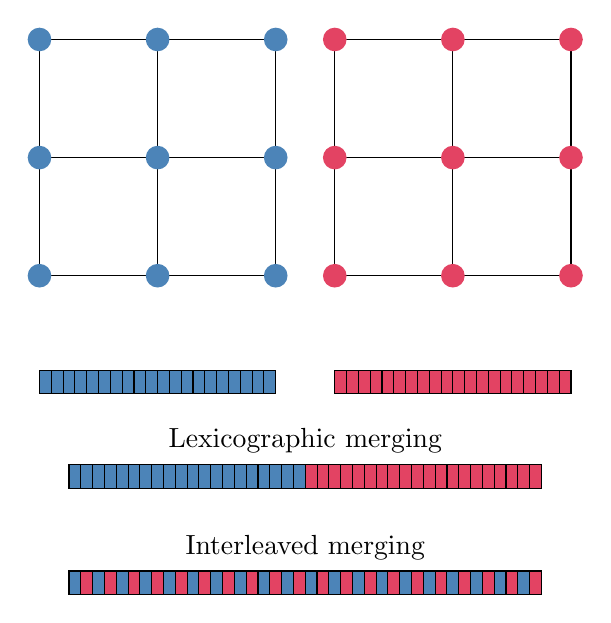
\begin{tikzpicture}[scale=1.5]

\colorlet{ca}{niceblue!80}
\colorlet{cb}{nicered!80}
\colorlet{cc}{niceorange!90}
\colorlet{cd}{niceviolet!60}

%%% Local Variables:
%%% mode: latex
%%% TeX-master: "../../diss-main"
%%% End:


\foreach \c / \i in {ca/0,cb/2.5}
{

\foreach \x in {0,1}
  \foreach \y in {0,1}
  {
    \draw (\x+4 + \i,\y) rectangle ++(1,1);
  }

\foreach \x in {0,1,2}
  \foreach \y in {0,1,2}
  {
    \fill[\c] (\x+4 + \i,\y) circle (0.1);
  }

\filldraw[fill=\c] (4 + \i,-1) rectangle ++(2,0.2);
\foreach \x in {0.1,0.2,...,1.9}
  \draw (4 + \i+\x,-1) -- ++(0,0.2);

\filldraw[fill=\c] ((4.25 + 0.8*\i,-1.8) rectangle ++(2,0.2);
 \foreach \x in {0.1,0.2,...,1.9}
   \draw (4.25 + 0.8*\i +\x,-1.8) -- ++(0,0.2);
}

\draw (6.25,-1.4) node {Lexicographic merging};

\draw (6.25,-2.3) node {Interleaved merging};

\foreach \x in {0,0.1,...,1.91}
{
  \fill[color=ca] (4.25+2*\x,-2.7) rectangle ++(0.1,0.2);
  \fill[color=cb] (4.35+2*\x,-2.7) rectangle ++(0.1,0.2);
}
\foreach \x in {0.1,0.2,...,3.9}
  \draw (4.25+\x,-2.7) -- ++(0,0.2);
\draw (4.25,-2.7) rectangle ++(4,0.2);

\end{tikzpicture}


%%% Local Variables:
%%% mode: latex
%%% TeX-master: "../../verteidigung"
%%% End:

}

    \end{column}
  \end{columns}
\end{frame}


\begin{frame}{Merging + Blocking}
  \begin{columns}
    \begin{column}{0.6\textwidth}
      \begin{itemize}
      \item Merging can be repeated at every tree node\\
{\small $\Rightarrow$ recursive construction of index structure from function space structure}
\item Also support \structure{blocking} during merging
{\small
  \begin{itemize}
  \item Large blocks for extracting subproblem matrices
  \item Small blocks for block-aware preconditioners and
    reduced memory usage
  \end{itemize}
}
      \end{itemize}
%\vspace*{2em}
\resizebox{\textwidth}{!}{
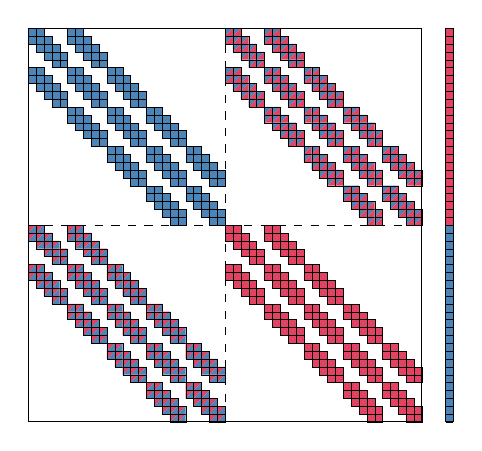
\begin{tikzpicture}

\colorlet{ca}{niceblue!80}
\colorlet{cb}{nicered!80}
\colorlet{cc}{niceorange!90}
\colorlet{cd}{niceviolet!60}

%%% Local Variables:
%%% mode: latex
%%% TeX-master: "../../diss-main"
%%% End:


\foreach \x / \y in {0/0, 0/1, 0/5, 0/6, 1/0, 1/1, 1/2, 1/5, 1/6, 1/7, 2/1, 2/2, 2/3, 2/6, 2/7, 2/8, 3/2, 3/3, 3/4, 3/7, 3/8, 3/9, 4/3, 4/4, 4/8, 4/9, 5/0, 5/1, 5/5, 5/6, 5/10, 5/11, 6/0, 6/1, 6/2, 6/5, 6/6, 6/7, 6/10, 6/11, 6/12, 7/1, 7/2, 7/3, 7/6, 7/7, 7/8, 7/11, 7/12, 7/13, 8/2, 8/3, 8/4, 8/7, 8/8, 8/9, 8/12, 8/13, 8/14, 9/3, 9/4, 9/8, 9/9, 9/13, 9/14, 10/5, 10/6, 10/10, 10/11, 10/15, 10/16, 11/5, 11/6, 11/7, 11/10, 11/11, 11/12, 11/15, 11/16, 11/17, 12/6, 12/7, 12/8, 12/11, 12/12, 12/13, 12/16, 12/17, 12/18, 13/7, 13/8, 13/9, 13/12, 13/13, 13/14, 13/17, 13/18, 13/19, 14/8, 14/9, 14/13, 14/14, 14/18, 14/19, 15/10, 15/11, 15/15, 15/16, 15/20, 15/21, 16/10, 16/11, 16/12, 16/15, 16/16, 16/17, 16/20, 16/21, 16/22, 17/11, 17/12, 17/13, 17/16, 17/17, 17/18, 17/21, 17/22, 17/23, 18/12, 18/13, 18/14, 18/17, 18/18, 18/19, 18/22, 18/23, 18/24, 19/13, 19/14, 19/18, 19/19, 19/23, 19/24, 20/15, 20/16, 20/20, 20/21, 21/15, 21/16, 21/17, 21/20, 21/21, 21/22, 22/16, 22/17, 22/18, 22/21, 22/22, 22/23, 23/17, 23/18, 23/19, 23/22, 23/23, 23/24, 24/18, 24/19, 24/23, 24/24}
{
  \filldraw[fill=ca,ultra thin] (0.1*\x,-0.1*\y) rectangle ++(0.1,-0.1);
}

\foreach \x / \y in {25/25, 25/26, 25/30, 25/31, 26/25, 26/26, 26/27, 26/30, 26/31, 26/32, 27/26, 27/27, 27/28, 27/31, 27/32, 27/33, 28/27, 28/28, 28/29, 28/32, 28/33, 28/34, 29/28, 29/29, 29/33, 29/34, 30/25, 30/26, 30/30, 30/31, 30/35, 30/36, 31/25, 31/26, 31/27, 31/30, 31/31, 31/32, 31/35, 31/36, 31/37, 32/26, 32/27, 32/28, 32/31, 32/32, 32/33, 32/36, 32/37, 32/38, 33/27, 33/28, 33/29, 33/32, 33/33, 33/34, 33/37, 33/38, 33/39, 34/28, 34/29, 34/33, 34/34, 34/38, 34/39, 35/30, 35/31, 35/35, 35/36, 35/40, 35/41, 36/30, 36/31, 36/32, 36/35, 36/36, 36/37, 36/40, 36/41, 36/42, 37/31, 37/32, 37/33, 37/36, 37/37, 37/38, 37/41, 37/42, 37/43, 38/32, 38/33, 38/34, 38/37, 38/38, 38/39, 38/42, 38/43, 38/44, 39/33, 39/34, 39/38, 39/39, 39/43, 39/44, 40/35, 40/36, 40/40, 40/41, 40/45, 40/46, 41/35, 41/36, 41/37, 41/40, 41/41, 41/42, 41/45, 41/46, 41/47, 42/36, 42/37, 42/38, 42/41, 42/42, 42/43, 42/46, 42/47, 42/48, 43/37, 43/38, 43/39, 43/42, 43/43, 43/44, 43/47, 43/48, 43/49, 44/38, 44/39, 44/43, 44/44, 44/48, 44/49, 45/40, 45/41, 45/45, 45/46, 46/40, 46/41, 46/42, 46/45, 46/46, 46/47, 47/41, 47/42, 47/43, 47/46, 47/47, 47/48, 48/42, 48/43, 48/44, 48/47, 48/48, 48/49, 49/43, 49/44, 49/48, 49/49}
{
  \filldraw[fill=cb,ultra thin] (0.1*\x,-0.1*\y) rectangle ++(0.1,-0.1);
}

\foreach \x / \y in {0/25, 0/26, 0/30, 0/31, 1/25, 1/26, 1/27, 1/30, 1/31, 1/32, 2/26, 2/27, 2/28, 2/31, 2/32, 2/33, 3/27, 3/28, 3/29, 3/32, 3/33, 3/34, 4/28, 4/29, 4/33, 4/34, 5/25, 5/26, 5/30, 5/31, 5/35, 5/36, 6/25, 6/26, 6/27, 6/30, 6/31, 6/32, 6/35, 6/36, 6/37, 7/26, 7/27, 7/28, 7/31, 7/32, 7/33, 7/36, 7/37, 7/38, 8/27, 8/28, 8/29, 8/32, 8/33, 8/34, 8/37, 8/38, 8/39, 9/28, 9/29, 9/33, 9/34, 9/38, 9/39, 10/30, 10/31, 10/35, 10/36, 10/40, 10/41, 11/30, 11/31, 11/32, 11/35, 11/36, 11/37, 11/40, 11/41, 11/42, 12/31, 12/32, 12/33, 12/36, 12/37, 12/38, 12/41, 12/42, 12/43, 13/32, 13/33, 13/34, 13/37, 13/38, 13/39, 13/42, 13/43, 13/44, 14/33, 14/34, 14/38, 14/39, 14/43, 14/44, 15/35, 15/36, 15/40, 15/41, 15/45, 15/46, 16/35, 16/36, 16/37, 16/40, 16/41, 16/42, 16/45, 16/46, 16/47, 17/36, 17/37, 17/38, 17/41, 17/42, 17/43, 17/46, 17/47, 17/48, 18/37, 18/38, 18/39, 18/42, 18/43, 18/44, 18/47, 18/48, 18/49, 19/38, 19/39, 19/43, 19/44, 19/48, 19/49, 20/40, 20/41, 20/45, 20/46, 21/40, 21/41, 21/42, 21/45, 21/46, 21/47, 22/41, 22/42, 22/43, 22/46, 22/47, 22/48, 23/42, 23/43, 23/44, 23/47, 23/48, 23/49, 24/43, 24/44, 24/48, 24/49}
{
  \fill[cb] (0.1*\x,-0.1*\y) -- ++(0.1,0) -- ++(-0.1,-0.1) --cycle;
  \fill[ca] (0.1*\x+0.1,-0.1*\y) -- ++(0,-0.1) -- ++(-0.1,0) --cycle;
  \draw[ultra thin] (0.1*\x,-0.1*\y) rectangle ++(0.1,-0.1);
}

\foreach \x / \y in {25/0, 25/1, 25/5, 25/6, 26/0, 26/1, 26/2, 26/5, 26/6, 26/7, 27/1, 27/2, 27/3, 27/6, 27/7, 27/8, 28/2, 28/3, 28/4, 28/7, 28/8, 28/9, 29/3, 29/4, 29/8, 29/9, 30/0, 30/1, 30/5, 30/6, 30/10, 30/11, 31/0, 31/1, 31/2, 31/5, 31/6, 31/7, 31/10, 31/11, 31/12, 32/1, 32/2, 32/3, 32/6, 32/7, 32/8, 32/11, 32/12, 32/13, 33/2, 33/3, 33/4, 33/7, 33/8, 33/9, 33/12, 33/13, 33/14, 34/3, 34/4, 34/8, 34/9, 34/13, 34/14, 35/5, 35/6, 35/10, 35/11, 35/15, 35/16, 36/5, 36/6, 36/7, 36/10, 36/11, 36/12, 36/15, 36/16, 36/17, 37/6, 37/7, 37/8, 37/11, 37/12, 37/13, 37/16, 37/17, 37/18, 38/7, 38/8, 38/9, 38/12, 38/13, 38/14, 38/17, 38/18, 38/19, 39/8, 39/9, 39/13, 39/14, 39/18, 39/19, 40/10, 40/11, 40/15, 40/16, 40/20, 40/21, 41/10, 41/11, 41/12, 41/15, 41/16, 41/17, 41/20, 41/21, 41/22, 42/11, 42/12, 42/13, 42/16, 42/17, 42/18, 42/21, 42/22, 42/23, 43/12, 43/13, 43/14, 43/17, 43/18, 43/19, 43/22, 43/23, 43/24, 44/13, 44/14, 44/18, 44/19, 44/23, 44/24, 45/15, 45/16, 45/20, 45/21, 46/15, 46/16, 46/17, 46/20, 46/21, 46/22, 47/16, 47/17, 47/18, 47/21, 47/22, 47/23, 48/17, 48/18, 48/19, 48/22, 48/23, 48/24, 49/18, 49/19, 49/23, 49/24}
{
  \fill[ca] (0.1*\x,-0.1*\y) -- ++(0.1,0) -- ++(-0.1,-0.1) --cycle;
  \fill[cb] (0.1*\x+0.1,-0.1*\y) -- ++(0,-0.1) -- ++(-0.1,0) --cycle;
  \draw[ultra thin] (0.1*\x,-0.1*\y) rectangle ++(0.1,-0.1);
}

\fill[cb] (5.3,0) rectangle ++(0.1,-2.5);
\fill[ca] (5.3,-2.5) rectangle ++(0.1,-2.5);
\draw (5.3,0) rectangle ++(0.1,-5);

\foreach \x in {0,1,...,50}
{
  %\draw (0.1*\x,0) -- ++(0,-5);
  %\draw (0,-0.1*\x) -- ++(5,0);
  \draw[ultra thin] (5.3,-0.1*\x) -- ++(0.1,0);
}

\draw (0,0) rectangle (5,-5);

\draw[dashed,very thin]
  (0,-2.5) -- (5,-2.5)
  (2.5,0) -- (2.5,-5);

\end{tikzpicture}


%%% Local Variables:
%%% mode: latex
%%% TeX-master: "../../diss-main"
%%% End:

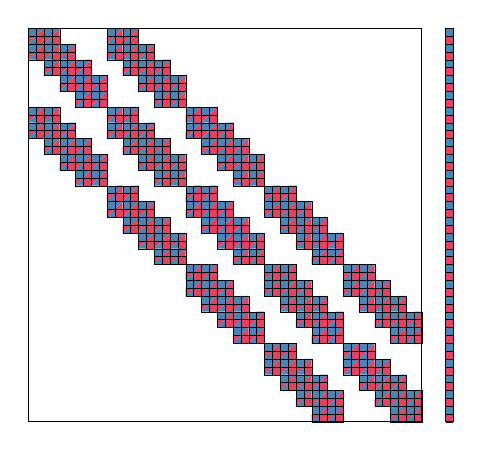
\begin{tikzpicture}

\colorlet{ca}{niceblue!80}
\colorlet{cb}{nicered!80}
\colorlet{cc}{niceorange!90}
\colorlet{cd}{niceviolet!60}

%%% Local Variables:
%%% mode: latex
%%% TeX-master: "../../diss-main"
%%% End:


\foreach \x / \y in {0/0, 0/2, 0/10, 0/12, 2/0, 2/2, 2/4, 2/10,
  2/12, 2/14, 4/2, 4/4, 4/6, 4/12, 4/14, 4/16, 6/4, 6/6, 6/8,
  6/14, 6/16, 6/18, 8/6, 8/8, 8/16, 8/18, 10/0, 10/2, 10/10,
  10/12, 10/20, 10/22, 12/0, 12/2, 12/4, 12/10, 12/12, 12/14,
  12/20, 12/22, 12/24, 14/2, 14/4, 14/6, 14/12, 14/14, 14/16,
  14/22, 14/24, 14/26, 16/4, 16/6, 16/8, 16/14, 16/16, 16/18,
  16/24, 16/26, 16/28, 18/6, 18/8, 18/16, 18/18, 18/26, 18/28,
  20/10, 20/12, 20/20, 20/22, 20/30, 20/32, 22/10, 22/12, 22/14,
  22/20, 22/22, 22/24, 22/30, 22/32, 22/34, 24/12, 24/14, 24/16,
  24/22, 24/24, 24/26, 24/32, 24/34, 24/36, 26/14, 26/16, 26/18,
  26/24, 26/26, 26/28, 26/34, 26/36, 26/38, 28/16, 28/18, 28/26,
  28/28, 28/36, 28/38, 30/20, 30/22, 30/30, 30/32, 30/40, 30/42,
  32/20, 32/22, 32/24, 32/30, 32/32, 32/34, 32/40, 32/42, 32/44,
  34/22, 34/24, 34/26, 34/32, 34/34, 34/36, 34/42, 34/44, 34/46,
  36/24, 36/26, 36/28, 36/34, 36/36, 36/38, 36/44, 36/46, 36/48,
  38/26, 38/28, 38/36, 38/38, 38/46, 38/48, 40/30, 40/32, 40/40,
  40/42, 42/30, 42/32, 42/34, 42/40, 42/42, 42/44, 44/32, 44/34,
  44/36, 44/42, 44/44, 44/46, 46/34, 46/36, 46/38, 46/44, 46/46,
  46/48, 48/36, 48/38, 48/46, 48/48}
{
  \filldraw[fill=ca,ultra thin] (0.1*\x,-0.1*\y) rectangle ++(0.1,-0.1);
}

\foreach \x / \y in {1/1, 1/3, 1/11, 1/13, 3/1, 3/3, 3/5, 3/11,
  3/13, 3/15, 5/3, 5/5, 5/7, 5/13, 5/15, 5/17, 7/5, 7/7, 7/9,
  7/15, 7/17, 7/19, 9/7, 9/9, 9/17, 9/19, 11/1, 11/3, 11/11,
  11/13, 11/21, 11/23, 13/1, 13/3, 13/5, 13/11, 13/13, 13/15,
  13/21, 13/23, 13/25, 15/3, 15/5, 15/7, 15/13, 15/15, 15/17,
  15/23, 15/25, 15/27, 17/5, 17/7, 17/9, 17/15, 17/17, 17/19,
  17/25, 17/27, 17/29, 19/7, 19/9, 19/17, 19/19, 19/27, 19/29,
  21/11, 21/13, 21/21, 21/23, 21/31, 21/33, 23/11, 23/13, 23/15,
  23/21, 23/23, 23/25, 23/31, 23/33, 23/35, 25/13, 25/15, 25/17,
  25/23, 25/25, 25/27, 25/33, 25/35, 25/37, 27/15, 27/17, 27/19,
  27/25, 27/27, 27/29, 27/35, 27/37, 27/39, 29/17, 29/19, 29/27,
  29/29, 29/37, 29/39, 31/21, 31/23, 31/31, 31/33, 31/41, 31/43,
  33/21, 33/23, 33/25, 33/31, 33/33, 33/35, 33/41, 33/43, 33/45,
  35/23, 35/25, 35/27, 35/33, 35/35, 35/37, 35/43, 35/45, 35/47,
  37/25, 37/27, 37/29, 37/35, 37/37, 37/39, 37/45, 37/47, 37/49,
  39/27, 39/29, 39/37, 39/39, 39/47, 39/49, 41/31, 41/33, 41/41,
  41/43, 43/31, 43/33, 43/35, 43/41, 43/43, 43/45, 45/33, 45/35,
  45/37, 45/43, 45/45, 45/47, 47/35, 47/37, 47/39, 47/45, 47/47,
  47/49, 49/37, 49/39, 49/47, 49/49}
{
  \filldraw[fill=cb,ultra thin] (0.1*\x,-0.1*\y) rectangle ++(0.1,-0.1);
}

\foreach \x / \y in {0/1, 0/3, 0/11, 0/13, 2/1, 2/3, 2/5, 2/11,
  2/13, 2/15, 4/3, 4/5, 4/7, 4/13, 4/15, 4/17, 6/5, 6/7, 6/9,
  6/15, 6/17, 6/19, 8/7, 8/9, 8/17, 8/19, 10/1, 10/3, 10/11,
  10/13, 10/21, 10/23, 12/1, 12/3, 12/5, 12/11, 12/13, 12/15,
  12/21, 12/23, 12/25, 14/3, 14/5, 14/7, 14/13, 14/15, 14/17,
  14/23, 14/25, 14/27, 16/5, 16/7, 16/9, 16/15, 16/17, 16/19,
  16/25, 16/27, 16/29, 18/7, 18/9, 18/17, 18/19, 18/27, 18/29,
  20/11, 20/13, 20/21, 20/23, 20/31, 20/33, 22/11, 22/13, 22/15,
  22/21, 22/23, 22/25, 22/31, 22/33, 22/35, 24/13, 24/15, 24/17,
  24/23, 24/25, 24/27, 24/33, 24/35, 24/37, 26/15, 26/17, 26/19,
  26/25, 26/27, 26/29, 26/35, 26/37, 26/39, 28/17, 28/19, 28/27,
  28/29, 28/37, 28/39, 30/21, 30/23, 30/31, 30/33, 30/41, 30/43,
  32/21, 32/23, 32/25, 32/31, 32/33, 32/35, 32/41, 32/43, 32/45,
  34/23, 34/25, 34/27, 34/33, 34/35, 34/37, 34/43, 34/45, 34/47,
  36/25, 36/27, 36/29, 36/35, 36/37, 36/39, 36/45, 36/47, 36/49,
  38/27, 38/29, 38/37, 38/39, 38/47, 38/49, 40/31, 40/33, 40/41,
  40/43, 42/31, 42/33, 42/35, 42/41, 42/43, 42/45, 44/33, 44/35,
  44/37, 44/43, 44/45, 44/47, 46/35, 46/37, 46/39, 46/45, 46/47,
  46/49, 48/37, 48/39, 48/47, 48/49}
{
  \fill[cb] (0.1*\x,-0.1*\y) -- ++(0.1,0) -- ++(-0.1,-0.1) --cycle;
  \fill[ca] (0.1*\x+0.1,-0.1*\y) -- ++(0,-0.1) -- ++(-0.1,0) --cycle;
  \draw[ultra thin] (0.1*\x,-0.1*\y) rectangle ++(0.1,-0.1);
}

\foreach \x / \y in {1/0, 1/2, 1/10, 1/12, 3/0, 3/2, 3/4, 3/10,
  3/12, 3/14, 5/2, 5/4, 5/6, 5/12, 5/14, 5/16, 7/4, 7/6, 7/8,
  7/14, 7/16, 7/18, 9/6, 9/8, 9/16, 9/18, 11/0, 11/2, 11/10,
  11/12, 11/20, 11/22, 13/0, 13/2, 13/4, 13/10, 13/12, 13/14,
  13/20, 13/22, 13/24, 15/2, 15/4, 15/6, 15/12, 15/14, 15/16,
  15/22, 15/24, 15/26, 17/4, 17/6, 17/8, 17/14, 17/16, 17/18,
  17/24, 17/26, 17/28, 19/6, 19/8, 19/16, 19/18, 19/26, 19/28,
  21/10, 21/12, 21/20, 21/22, 21/30, 21/32, 23/10, 23/12, 23/14,
  23/20, 23/22, 23/24, 23/30, 23/32, 23/34, 25/12, 25/14, 25/16,
  25/22, 25/24, 25/26, 25/32, 25/34, 25/36, 27/14, 27/16, 27/18,
  27/24, 27/26, 27/28, 27/34, 27/36, 27/38, 29/16, 29/18, 29/26,
  29/28, 29/36, 29/38, 31/20, 31/22, 31/30, 31/32, 31/40, 31/42,
  33/20, 33/22, 33/24, 33/30, 33/32, 33/34, 33/40, 33/42, 33/44,
  35/22, 35/24, 35/26, 35/32, 35/34, 35/36, 35/42, 35/44, 35/46,
  37/24, 37/26, 37/28, 37/34, 37/36, 37/38, 37/44, 37/46, 37/48,
  39/26, 39/28, 39/36, 39/38, 39/46, 39/48, 41/30, 41/32, 41/40,
  41/42, 43/30, 43/32, 43/34, 43/40, 43/42, 43/44, 45/32, 45/34,
  45/36, 45/42, 45/44, 45/46, 47/34, 47/36, 47/38, 47/44, 47/46,
  47/48, 49/36, 49/38, 49/46, 49/48}
{
  \fill[ca] (0.1*\x,-0.1*\y) -- ++(0.1,0) -- ++(-0.1,-0.1) --cycle;
  \fill[cb] (0.1*\x+0.1,-0.1*\y) -- ++(0,-0.1) -- ++(-0.1,0) --cycle;
  \draw[ultra thin] (0.1*\x,-0.1*\y) rectangle ++(0.1,-0.1);
}

\foreach \x in {0,1,...,24}
{
  \fill[ca] (5.3,-0.2*\x) rectangle ++(0.1,-0.1);
  \fill[cb] (5.3,-0.2*\x-0.1) rectangle ++(0.1,-0.1);
}

\draw (5.3,0) rectangle ++(0.1,-5);

\foreach \x in {0,1,...,50}
{
  %\draw (0.1*\x,0) -- ++(0,-5);
  %\draw (0,-0.1*\x) -- ++(5,0);
  \draw[ultra thin] (5.3,-0.1*\x) -- ++(0.1,0);
}

\draw (0,0) rectangle (5,-5);

\end{tikzpicture}


%%% Local Variables:
%%% mode: latex
%%% TeX-master: "../../diss-main"
%%% End:

}
    \end{column}
    \begin{column}{0.4\textwidth}
\resizebox{0.8\textwidth}{!}{
  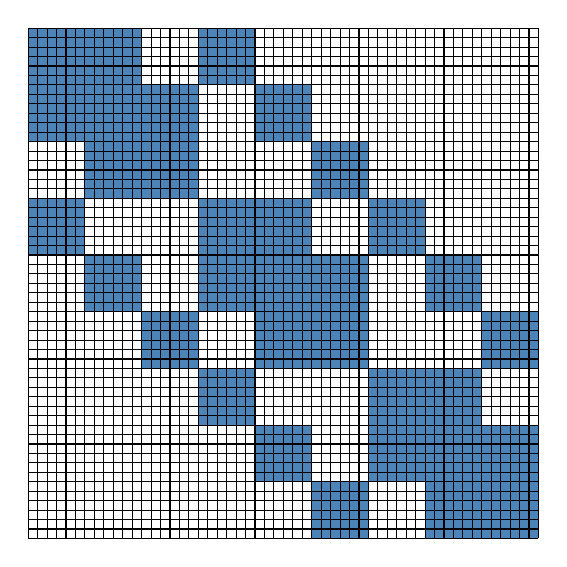
\begin{tikzpicture}[scale=1.2]

\colorlet{ca}{niceblue!80}
\colorlet{cb}{nicered!80}
\colorlet{cc}{niceorange!90}
\colorlet{cd}{niceviolet!60}

%%% Local Variables:
%%% mode: latex
%%% TeX-master: "../../diss-main"
%%% End:


\foreach \x / \y in {0/0, 0/1, 0/2, 0/3, 0/4, 0/5, 0/6, 0/7, 0/8,
  0/9, 0/10, 0/11, 0/18, 0/19, 0/20, 0/21, 0/22, 0/23, 1/0, 1/1,
  1/2, 1/3, 1/4, 1/5, 1/6, 1/7, 1/8, 1/9, 1/10, 1/11, 1/18, 1/19,
  1/20, 1/21, 1/22, 1/23, 2/0, 2/1, 2/2, 2/3, 2/4, 2/5, 2/6, 2/7,
  2/8, 2/9, 2/10, 2/11, 2/18, 2/19, 2/20, 2/21, 2/22, 2/23, 3/0,
  3/1, 3/2, 3/3, 3/4, 3/5, 3/6, 3/7, 3/8, 3/9, 3/10, 3/11, 3/18,
  3/19, 3/20, 3/21, 3/22, 3/23, 4/0, 4/1, 4/2, 4/3, 4/4, 4/5, 4/6,
  4/7, 4/8, 4/9, 4/10, 4/11, 4/18, 4/19, 4/20, 4/21, 4/22, 4/23,
  5/0, 5/1, 5/2, 5/3, 5/4, 5/5, 5/6, 5/7, 5/8, 5/9, 5/10, 5/11,
  5/18, 5/19, 5/20, 5/21, 5/22, 5/23, 6/0, 6/1, 6/2, 6/3, 6/4,
  6/5, 6/6, 6/7, 6/8, 6/9, 6/10, 6/11, 6/12, 6/13, 6/14, 6/15,
  6/16, 6/17, 6/24, 6/25, 6/26, 6/27, 6/28, 6/29, 7/0, 7/1, 7/2,
  7/3, 7/4, 7/5, 7/6, 7/7, 7/8, 7/9, 7/10, 7/11, 7/12, 7/13, 7/14,
  7/15, 7/16, 7/17, 7/24, 7/25, 7/26, 7/27, 7/28, 7/29, 8/0, 8/1,
  8/2, 8/3, 8/4, 8/5, 8/6, 8/7, 8/8, 8/9, 8/10, 8/11, 8/12, 8/13,
  8/14, 8/15, 8/16, 8/17, 8/24, 8/25, 8/26, 8/27, 8/28, 8/29, 9/0,
  9/1, 9/2, 9/3, 9/4, 9/5, 9/6, 9/7, 9/8, 9/9, 9/10, 9/11, 9/12,
  9/13, 9/14, 9/15, 9/16, 9/17, 9/24, 9/25, 9/26, 9/27, 9/28,
  9/29, 10/0, 10/1, 10/2, 10/3, 10/4, 10/5, 10/6, 10/7, 10/8,
  10/9, 10/10, 10/11, 10/12, 10/13, 10/14, 10/15, 10/16, 10/17,
  10/24, 10/25, 10/26, 10/27, 10/28, 10/29, 11/0, 11/1, 11/2,
  11/3, 11/4, 11/5, 11/6, 11/7, 11/8, 11/9, 11/10, 11/11, 11/12,
  11/13, 11/14, 11/15, 11/16, 11/17, 11/24, 11/25, 11/26, 11/27,
  11/28, 11/29, 12/6, 12/7, 12/8, 12/9, 12/10, 12/11, 12/12,
  12/13, 12/14, 12/15, 12/16, 12/17, 12/30, 12/31, 12/32, 12/33,
  12/34, 12/35, 13/6, 13/7, 13/8, 13/9, 13/10, 13/11, 13/12,
  13/13, 13/14, 13/15, 13/16, 13/17, 13/30, 13/31, 13/32, 13/33,
  13/34, 13/35, 14/6, 14/7, 14/8, 14/9, 14/10, 14/11, 14/12,
  14/13, 14/14, 14/15, 14/16, 14/17, 14/30, 14/31, 14/32, 14/33,
  14/34, 14/35, 15/6, 15/7, 15/8, 15/9, 15/10, 15/11, 15/12,
  15/13, 15/14, 15/15, 15/16, 15/17, 15/30, 15/31, 15/32, 15/33,
  15/34, 15/35, 16/6, 16/7, 16/8, 16/9, 16/10, 16/11, 16/12,
  16/13, 16/14, 16/15, 16/16, 16/17, 16/30, 16/31, 16/32, 16/33,
  16/34, 16/35, 17/6, 17/7, 17/8, 17/9, 17/10, 17/11, 17/12,
  17/13, 17/14, 17/15, 17/16, 17/17, 17/30, 17/31, 17/32, 17/33,
  17/34, 17/35, 18/0, 18/1, 18/2, 18/3, 18/4, 18/5, 18/18, 18/19,
  18/20, 18/21, 18/22, 18/23, 18/24, 18/25, 18/26, 18/27, 18/28,
  18/29, 18/36, 18/37, 18/38, 18/39, 18/40, 18/41, 19/0, 19/1,
  19/2, 19/3, 19/4, 19/5, 19/18, 19/19, 19/20, 19/21, 19/22,
  19/23, 19/24, 19/25, 19/26, 19/27, 19/28, 19/29, 19/36, 19/37,
  19/38, 19/39, 19/40, 19/41, 20/0, 20/1, 20/2, 20/3, 20/4, 20/5,
  20/18, 20/19, 20/20, 20/21, 20/22, 20/23, 20/24, 20/25, 20/26,
  20/27, 20/28, 20/29, 20/36, 20/37, 20/38, 20/39, 20/40, 20/41,
  21/0, 21/1, 21/2, 21/3, 21/4, 21/5, 21/18, 21/19, 21/20, 21/21,
  21/22, 21/23, 21/24, 21/25, 21/26, 21/27, 21/28, 21/29, 21/36,
  21/37, 21/38, 21/39, 21/40, 21/41, 22/0, 22/1, 22/2, 22/3, 22/4,
  22/5, 22/18, 22/19, 22/20, 22/21, 22/22, 22/23, 22/24, 22/25,
  22/26, 22/27, 22/28, 22/29, 22/36, 22/37, 22/38, 22/39, 22/40,
  22/41, 23/0, 23/1, 23/2, 23/3, 23/4, 23/5, 23/18, 23/19, 23/20,
  23/21, 23/22, 23/23, 23/24, 23/25, 23/26, 23/27, 23/28, 23/29,
  23/36, 23/37, 23/38, 23/39, 23/40, 23/41, 24/6, 24/7, 24/8,
  24/9, 24/10, 24/11, 24/18, 24/19, 24/20, 24/21, 24/22, 24/23,
  24/24, 24/25, 24/26, 24/27, 24/28, 24/29, 24/30, 24/31, 24/32,
  24/33, 24/34, 24/35, 24/42, 24/43, 24/44, 24/45, 24/46, 24/47,
  25/6, 25/7, 25/8, 25/9, 25/10, 25/11, 25/18, 25/19, 25/20,
  25/21, 25/22, 25/23, 25/24, 25/25, 25/26, 25/27, 25/28, 25/29,
  25/30, 25/31, 25/32, 25/33, 25/34, 25/35, 25/42, 25/43, 25/44,
  25/45, 25/46, 25/47, 26/6, 26/7, 26/8, 26/9, 26/10, 26/11,
  26/18, 26/19, 26/20, 26/21, 26/22, 26/23, 26/24, 26/25, 26/26,
  26/27, 26/28, 26/29, 26/30, 26/31, 26/32, 26/33, 26/34, 26/35,
  26/42, 26/43, 26/44, 26/45, 26/46, 26/47, 27/6, 27/7, 27/8,
  27/9, 27/10, 27/11, 27/18, 27/19, 27/20, 27/21, 27/22, 27/23,
  27/24, 27/25, 27/26, 27/27, 27/28, 27/29, 27/30, 27/31, 27/32,
  27/33, 27/34, 27/35, 27/42, 27/43, 27/44, 27/45, 27/46, 27/47,
  28/6, 28/7, 28/8, 28/9, 28/10, 28/11, 28/18, 28/19, 28/20,
  28/21, 28/22, 28/23, 28/24, 28/25, 28/26, 28/27, 28/28, 28/29,
  28/30, 28/31, 28/32, 28/33, 28/34, 28/35, 28/42, 28/43, 28/44,
  28/45, 28/46, 28/47, 29/6, 29/7, 29/8, 29/9, 29/10, 29/11,
  29/18, 29/19, 29/20, 29/21, 29/22, 29/23, 29/24, 29/25, 29/26,
  29/27, 29/28, 29/29, 29/30, 29/31, 29/32, 29/33, 29/34, 29/35,
  29/42, 29/43, 29/44, 29/45, 29/46, 29/47, 30/12, 30/13, 30/14,
  30/15, 30/16, 30/17, 30/24, 30/25, 30/26, 30/27, 30/28, 30/29,
  30/30, 30/31, 30/32, 30/33, 30/34, 30/35, 30/48, 30/49, 30/50,
  30/51, 30/52, 30/53, 31/12, 31/13, 31/14, 31/15, 31/16, 31/17,
  31/24, 31/25, 31/26, 31/27, 31/28, 31/29, 31/30, 31/31, 31/32,
  31/33, 31/34, 31/35, 31/48, 31/49, 31/50, 31/51, 31/52, 31/53,
  32/12, 32/13, 32/14, 32/15, 32/16, 32/17, 32/24, 32/25, 32/26,
  32/27, 32/28, 32/29, 32/30, 32/31, 32/32, 32/33, 32/34, 32/35,
  32/48, 32/49, 32/50, 32/51, 32/52, 32/53, 33/12, 33/13, 33/14,
  33/15, 33/16, 33/17, 33/24, 33/25, 33/26, 33/27, 33/28, 33/29,
  33/30, 33/31, 33/32, 33/33, 33/34, 33/35, 33/48, 33/49, 33/50,
  33/51, 33/52, 33/53, 34/12, 34/13, 34/14, 34/15, 34/16, 34/17,
  34/24, 34/25, 34/26, 34/27, 34/28, 34/29, 34/30, 34/31, 34/32,
  34/33, 34/34, 34/35, 34/48, 34/49, 34/50, 34/51, 34/52, 34/53,
  35/12, 35/13, 35/14, 35/15, 35/16, 35/17, 35/24, 35/25, 35/26,
  35/27, 35/28, 35/29, 35/30, 35/31, 35/32, 35/33, 35/34, 35/35,
  35/48, 35/49, 35/50, 35/51, 35/52, 35/53, 36/18, 36/19, 36/20,
  36/21, 36/22, 36/23, 36/36, 36/37, 36/38, 36/39, 36/40, 36/41,
  36/42, 36/43, 36/44, 36/45, 36/46, 36/47, 37/18, 37/19, 37/20,
  37/21, 37/22, 37/23, 37/36, 37/37, 37/38, 37/39, 37/40, 37/41,
  37/42, 37/43, 37/44, 37/45, 37/46, 37/47, 38/18, 38/19, 38/20,
  38/21, 38/22, 38/23, 38/36, 38/37, 38/38, 38/39, 38/40, 38/41,
  38/42, 38/43, 38/44, 38/45, 38/46, 38/47, 39/18, 39/19, 39/20,
  39/21, 39/22, 39/23, 39/36, 39/37, 39/38, 39/39, 39/40, 39/41,
  39/42, 39/43, 39/44, 39/45, 39/46, 39/47, 40/18, 40/19, 40/20,
  40/21, 40/22, 40/23, 40/36, 40/37, 40/38, 40/39, 40/40, 40/41,
  40/42, 40/43, 40/44, 40/45, 40/46, 40/47, 41/18, 41/19, 41/20,
  41/21, 41/22, 41/23, 41/36, 41/37, 41/38, 41/39, 41/40, 41/41,
  41/42, 41/43, 41/44, 41/45, 41/46, 41/47, 42/24, 42/25, 42/26,
  42/27, 42/28, 42/29, 42/36, 42/37, 42/38, 42/39, 42/40, 42/41,
  42/42, 42/43, 42/44, 42/45, 42/46, 42/47, 42/48, 42/49, 42/50,
  42/51, 42/52, 42/53, 43/24, 43/25, 43/26, 43/27, 43/28, 43/29,
  43/36, 43/37, 43/38, 43/39, 43/40, 43/41, 43/42, 43/43, 43/44,
  43/45, 43/46, 43/47, 43/48, 43/49, 43/50, 43/51, 43/52, 43/53,
  44/24, 44/25, 44/26, 44/27, 44/28, 44/29, 44/36, 44/37, 44/38,
  44/39, 44/40, 44/41, 44/42, 44/43, 44/44, 44/45, 44/46, 44/47,
  44/48, 44/49, 44/50, 44/51, 44/52, 44/53, 45/24, 45/25, 45/26,
  45/27, 45/28, 45/29, 45/36, 45/37, 45/38, 45/39, 45/40, 45/41,
  45/42, 45/43, 45/44, 45/45, 45/46, 45/47, 45/48, 45/49, 45/50,
  45/51, 45/52, 45/53, 46/24, 46/25, 46/26, 46/27, 46/28, 46/29,
  46/36, 46/37, 46/38, 46/39, 46/40, 46/41, 46/42, 46/43, 46/44,
  46/45, 46/46, 46/47, 46/48, 46/49, 46/50, 46/51, 46/52, 46/53,
  47/24, 47/25, 47/26, 47/27, 47/28, 47/29, 47/36, 47/37, 47/38,
  47/39, 47/40, 47/41, 47/42, 47/43, 47/44, 47/45, 47/46, 47/47,
  47/48, 47/49, 47/50, 47/51, 47/52, 47/53, 48/30, 48/31, 48/32,
  48/33, 48/34, 48/35, 48/42, 48/43, 48/44, 48/45, 48/46, 48/47,
  48/48, 48/49, 48/50, 48/51, 48/52, 48/53, 49/30, 49/31, 49/32,
  49/33, 49/34, 49/35, 49/42, 49/43, 49/44, 49/45, 49/46, 49/47,
  49/48, 49/49, 49/50, 49/51, 49/52, 49/53, 50/30, 50/31, 50/32,
  50/33, 50/34, 50/35, 50/42, 50/43, 50/44, 50/45, 50/46, 50/47,
  50/48, 50/49, 50/50, 50/51, 50/52, 50/53, 51/30, 51/31, 51/32,
  51/33, 51/34, 51/35, 51/42, 51/43, 51/44, 51/45, 51/46, 51/47,
  51/48, 51/49, 51/50, 51/51, 51/52, 51/53, 52/30, 52/31, 52/32,
  52/33, 52/34, 52/35, 52/42, 52/43, 52/44, 52/45, 52/46, 52/47,
  52/48, 52/49, 52/50, 52/51, 52/52, 52/53, 53/30, 53/31, 53/32,
  53/33, 53/34, 53/35, 53/42, 53/43, 53/44, 53/45, 53/46, 53/47,
  53/48, 53/49, 53/50, 53/51, 53/52, 53/53}
{
  \fill[ca] (0.1*\x,-0.1*\y) rectangle ++(0.1,-0.1);
}

\foreach \x in {0,1,...,54} { \draw (0.1*\x,0) -- ++(0,-5.4);
      \draw (0,-0.1*\x) -- ++(5.4,0); }

\end{tikzpicture}


%%% Local Variables:
%%% mode: latex
%%% TeX-master: "../../diss-main"
%%% End:

}
\ \\[1em]
\resizebox{0.8\textwidth}{!}{
  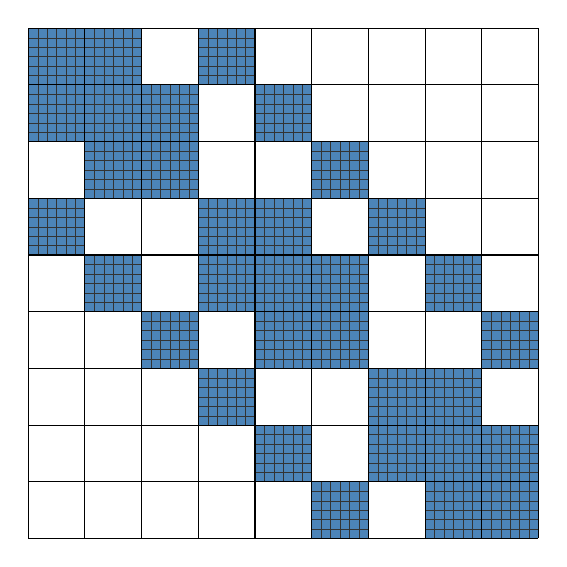
\begin{tikzpicture}[scale=1.2]

\colorlet{ca}{niceblue!80}
\colorlet{cb}{nicered!80}
\colorlet{cc}{niceorange!90}
\colorlet{cd}{niceviolet!60}

%%% Local Variables:
%%% mode: latex
%%% TeX-master: "../../diss-main"
%%% End:


\foreach \x / \y in {0/0, 0/6, 0/18, 6/0, 6/6, 6/12, 6/24, 12/6, 12/12, 12/30, 18/0, 18/18, 18/24, 18/36, 24/6, 24/18, 24/24, 24/30, 24/42, 30/12, 30/24, 30/30, 30/48, 36/18, 36/36, 36/42, 42/24, 42/36, 42/42, 42/48, 48/30, 48/42, 48/48}
{
  \fill[ca] (0.1*\x,-0.1*\y) rectangle ++(0.6,-0.6);
  \foreach \dx in {0.1,0.2,...,0.51}
  {
    \draw[black!80,ultra thin] (0.1*\x+\dx,-0.1*\y) -- ++(0,-0.6);
    \draw[black!80,ultra thin] (0.1*\x,-0.1*\y-\dx) -- ++(0.6,0);
  }
}

\foreach \x in {0,1,...,9}
{
  \draw (0.6*\x,0) -- ++(0,-5.4);
  \draw (0,-0.6*\x) -- ++(5.4,0);
}

\end{tikzpicture}


%%% Local Variables:
%%% mode: latex
%%% TeX-master: "../../diss-main"
%%% End:

}

    \end{column}
  \end{columns}
\end{frame}

\begin{frame}
\frametitle{Realization in PDELab}
\begin{enumerate}[1)]
\item The ini-file
\lstinline{tutorial04.ini} holds parameters
controlling the execution.
\item Main file \lstinline{tutorial04.cc} includes the necessary C++,
DUNE and PDELab header files;
contains \lstinline{main} function;
instantiates DUNE grid objects and calls the \lstinline{driver} function
\item Function \lstinline{driver} in file \lstinline{driver.hh} instantiates
the necessary PDELab classes and finally solves the problem.
\item File \lstinline{wavefem.hh} contains the local operator classes
\lstinline{WaveFEM} and \lstinline{WaveL2} realizing the spatial
and temporal residual forms.
\end{enumerate}
\end{frame}

\begin{frame}
\bibliographystyle{plain}
\bibliography{slides04.bib}
\end{frame}

\end{document}
